\section{Experiments}
\subsection{Experimental Setup and Benchmarks}
\label{sec:protocol}
To rigorously validate our cooperative detection framework against the claims in Sec.~\ref{sec:introduction}, we conduct comprehensive evaluations across two complementary benchmarks: the multi-vehicle simulation benchmark \textbf{OPV2V}~\cite{opv2v} for controlled pose noise stress-testing, and the real-world infrastructure-to-vehicle benchmark \textbf{DAIR-V2X}~\cite{dairv2x} for physical domain transferability.

\textbf{OPV2V benchmark and protocol.} On OPV2V, the official split provides 6,374 training, 1,980 validation, and 2,170 test frames. We follow the registered HEAL-derived multi-vehicle camera protocol with visibility filtering disabled. Up to five cooperating vehicles within 70\,m are included according to dataset membership. Targets are gathered from participating vehicles, deduplicated by identity, and evaluated in $x,y\in[-51.2,51.2]$\,m and $z\in[-3,1]$\,m in the reference frame without removing occluded objects.

\textbf{Evaluation metrics.} We report average precision (AP) at bird's-eye-view (BEV) intersection-over-union (IoU) thresholds 0.3, 0.5, and 0.7. Detection scores must exceed 0.2, and oriented NMS uses overlap 0.15. Following established practice in multi-view visual geometry~\cite{dust3r,vggt}, we decouple multi-view geometric detection from global metric scale ambiguity: detection is evaluated under scale-aligned AP by scaling ground-truth boxes to prediction scale at scoring time (yaw unchanged). No translation or rotation ground-truth alignment is applied to predicted-pose evaluations. Ground-truth-pose (GT) fusion evaluates detection under ideal inter-vehicle calibration, whereas Predicted-pose (Pred.) fusion tests end-to-end cooperation using poses estimated purely from images.

\textbf{Comparative baselines across paradigms.} We benchmark against representative methods spanning three distinct cooperative perception paradigms:
\begin{enumerate}
    \item \emph{Intermediate Feature Fusion:} \textbf{V2X-ViT}~\cite{v2xvit}, \textbf{AttFuse}~\cite{opv2v}, and \textbf{F-Cooper}~\cite{fcooper}, which warp intermediate BEV feature maps using external pose transforms.
    \item \emph{Two-Stage Box Registration:} \textbf{V2X-Reg++}~\cite{v2xreg}, \textbf{FreeAlign}~\cite{freealign}, and \textbf{Naive Late Fusion}, which detect 3D boxes locally and perform post-hoc point-set registration.
    \item \emph{Explicit Point-Cloud Reconstruction:} An image-derived \textbf{PointPillar} pipeline~\cite{pointpillars} lifting predicted dense depth into pseudo-point clouds for pillar-based detection.
    \item \emph{Direct Query Baseline and References:} \textbf{Direct Query}, our ablation baseline sharing the identical 4-epoch joint backbone with frozen weights but with depth and grouping severed; \textbf{HEAL Camera BEV}~\cite{heal}; and single-vehicle sensing baselines.
\end{enumerate}
All comparative baselines use the same 4-camera surround RGB input protocol without LiDAR; their checkpoints and implementations follow the recorded sources.

\begin{table*}[t]
\centering\small
\setlength{\tabcolsep}{4.8pt}
\caption{Macro-benchmarking across cooperative perception paradigms under varying cross-vehicle pose noise $k$ on the OPV2V test set (2,170 frames). Noise is injected into methods that consume externally supplied inter-vehicle poses; \method{} is the no-external-pose control. All methods use the same 4-camera surround-view RGB input protocol without LiDAR. Scale-aligned BEV AP$_{.5}$ (\%).}
\label{tab:robustness}
\begin{tabular}{llrrrrrr}\toprule
Paradigm & Method & $k=0$ & $k=1$ & $k=2$ & $k=4$ & $k=7$ & $k=10$\\\midrule
\textbf{Ours (No External Pose)} & \textbf{\method{} (Pred., No External Pose)} & 44.52 & 44.52 & \textbf{44.52} & \textbf{44.52} & \textbf{44.52} & \textbf{44.52}\\
Oracle GT-Pose Control & \method{} (GT Pose) & 59.05 & 59.05 & 59.05 & 59.05 & 59.05 & 59.05\\\midrule
Intermediate Feature Fusion & V2X-ViT~\cite{v2xvit} & \textbf{60.35} & \textbf{56.16} & 45.03 & 29.46 & 20.28 & 16.78\\
Intermediate Feature Fusion & AttFuse~\cite{opv2v} & 52.90 & 49.56 & 41.09 & 28.11 & 21.38 & 19.32\\
Intermediate Feature Fusion & F-Cooper~\cite{fcooper} & 46.95 & 43.40 & 34.59 & 23.57 & 18.09 & 16.34\\\midrule
Two-Stage Box Registration & Naive Late Fusion (GT Pose) & 32.68 & 32.68 & 32.68 & 32.68 & 32.68 & 32.68\\
Two-Stage Box Registration & No-Correction (Late Fusion) & 32.68 & 29.94 & 22.36 & 11.72 & 8.16 & 7.94\\
Two-Stage Box Registration & V2X-Reg++~\cite{v2xreg} & 28.19 & 25.90 & 19.65 & 10.72 & 7.67 & 7.59\\
Two-Stage Box Registration & FreeAlign~\cite{freealign} & 28.18 & 25.82 & 19.41 & 10.59 & 7.80 & 7.79\\\midrule
Single-Vehicle Reference & Single Local (40\,m FOV) & 30.20 & 30.20 & 30.20 & 30.20 & 30.20 & 30.20\\
Single-Vehicle Reference & Single Global (70\,m ROI) & 13.29 & 13.29 & 13.29 & 13.29 & 13.29 & 13.29\\\bottomrule
\end{tabular}
\end{table*}

\subsection{Macro-Benchmarking: Overcoming Pose Noise and Misregistration}
\label{sec:robustness}
Addressing our first core claim, we evaluate vulnerability to external positioning noise. In intelligent transportation networks, GNSS multipath, satellite occlusions, and latency introduce substantial coordinate deviations. We benchmark \method{} against intermediate fusion and two-stage box-registration models on the OPV2V test protocol under six reported Gaussian noise levels $k \in \{0, 1, 2, 4, 7, 10\}$ ($\sigma_t = 0.2k$\,m, $\sigma_r = 0.2k^\circ$). The perturbation is applied only to methods that consume an external inter-vehicle pose; \method{} does not consume this input at inference.

As shown in Table~\ref{tab:robustness}, the results support three protocol-scoped observations:

\textbf{1. Catastrophic collapse of intermediate feature fusion.} Under idealized zero-noise conditions ($k=0$), V2X-ViT achieves 60.35\% AP$_{.5}$. However, its accuracy plummets monotonically as noise increases, dropping by 72.2\% to 16.78\% at $k=10$. This fragility is consistent with grid-level misalignment: intermediate fusion warps dense BEV features using the external pose transform, so spatial deviations scatter cross-attention weights and corrupt coherent feature representations. On the reported grid, \method{} crosses V2X-ViT between $k=2$ and $k=4$; this interval does not represent a directly evaluated intermediate noise level.

\textbf{2. Negative collaborative gain regime ($k \ge 4$).} When pose noise reaches $k \ge 4$ ($\sigma_t \ge 0.8$\,m), all intermediate fusion models fall below the single-vehicle local baseline (30.20\% AP$_{.5}$). Under severe misregistration, collaborating vehicles inject corrupted spatial cues into the ego coordinate frame, generating duplicate ghost detections that degrade performance below uncoordinated local sensing.

\textbf{3. Inherent bottleneck of two-stage box registration.} Exchanging 3D bounding boxes and performing post-hoc registration via point-set matching~\cite{v2xreg,freealign} does not solve this problem under the present protocol. Due to monocular depth uncertainty at extended ranges ($>30$\,m), single-vehicle detectors suffer false negatives; consequently, even with ground-truth pose alignment, Naive Late Fusion reaches a protocol-specific ceiling of 32.68\% AP$_{.5}$ (compared to 60.35\% for multi-view feature fusion). Under larger initial perturbations, geometric correspondence algorithms also produce false positives, with V2X-Reg++ and FreeAlign reaching approximately 7.6\% AP$_{.5}$ at $k=10$.

In contrast, \method{} directly infers multi-view visual geometry without externally supplied poses or brittle box matching, remaining at 44.52\% AP$_{.5}$ across the reported grid. Its margin over V2X-Reg++ ranges from 16.33 percentage points at $k=0$ to 36.93 percentage points at $k=10$; the margin over Naive Late Fusion with GT pose is 11.84 percentage points.

\subsection{Qualitative Analysis}
\label{sec:qualitative}
Figure~\ref{fig:qualitative} provides a representative multi-vehicle test scene for visual inspection. The single-vehicle prediction misses targets that are visible from the partner view. Under $k=2$, V2X-ViT introduces displaced and ghost boxes after feature warping, while the two-stage registration baseline retains larger residual box errors. \method{} preserves the shared target layout and produces boxes closer to the green ground-truth boxes in both the ego and partner views. This example is illustrative rather than an additional aggregate metric; it complements the full-test-set statistics in Table~\ref{tab:robustness}.

\begin{figure*}[t]
\centering
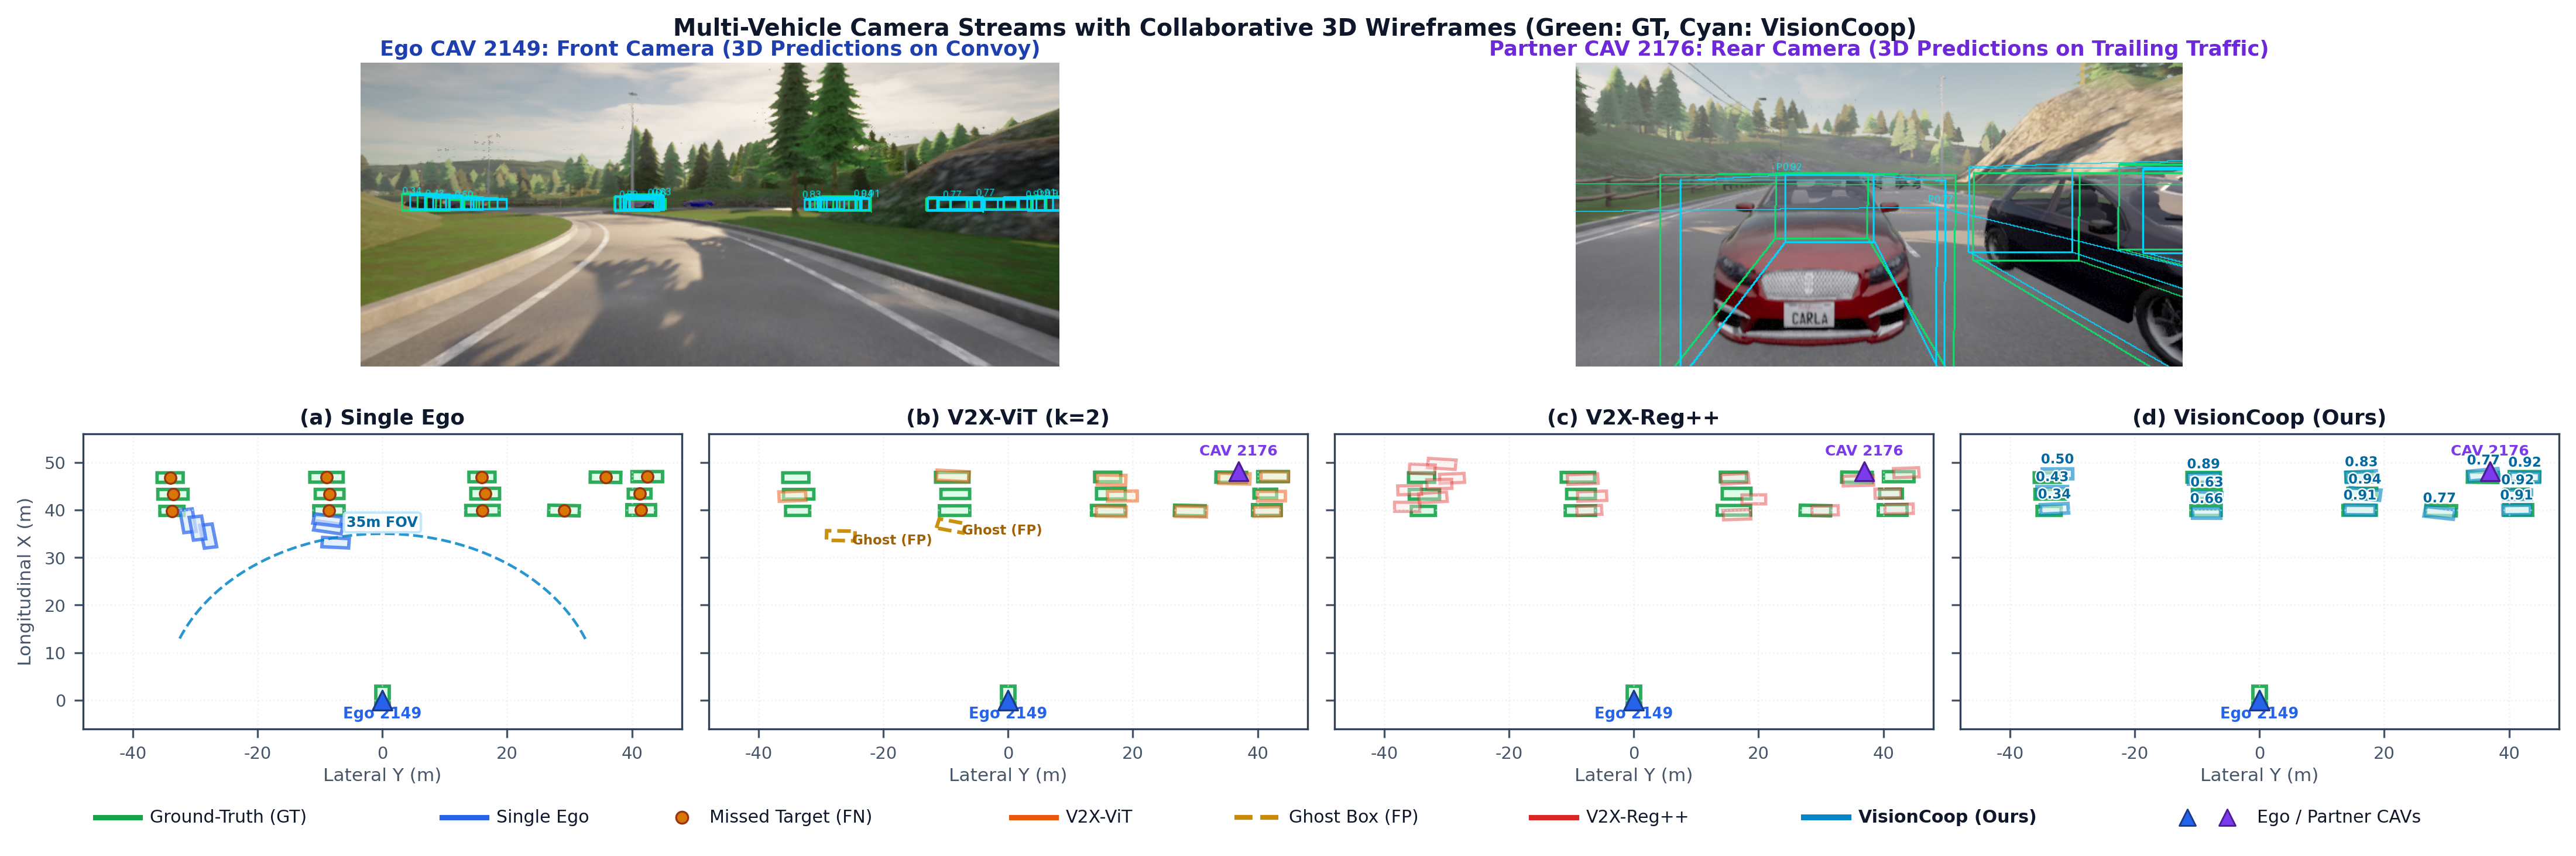
\includegraphics[width=\textwidth]{figures/qualitative_visualization.png}
\caption{Qualitative multi-vehicle comparison on a representative test scene. Green boxes denote ground truth and cyan boxes denote \method{} predictions; the lower panels compare single-ego sensing, V2X-ViT under $k=2$, V2X-Reg++, and \method{}. The visualization highlights missed targets and ghost boxes under misregistration and the improved cross-view consistency of the proposed query route.}
\label{fig:qualitative}
\end{figure*}

\begin{table}[t]
\centering\footnotesize
\setlength{\tabcolsep}{3pt}
\caption{Interface-level comparison of 3D detection routes on OPV2V test and validation splits. Scale-aligned BEV AP (\%). The rows use the recorded checkpoints and are not a fully matched single-factor ablation.}
\label{tab:main}
\begin{tabular}{llrrr}\toprule
Detection Route & Fusion & AP$_{.3}$ & AP$_{.5}$ & AP$_{.7}$\\\midrule
\multicolumn{5}{l}{\textit{Test Split:}} \\
HEAL Camera BEV~\cite{heal} & GT & 54.01 & 39.73 & 19.83\\
Direct Query (No Depth) & GT & 69.54 & 51.74 & 18.42\\
+ Naive Scalar Depth & GT & 52.19 & 39.37 & 11.20\\
PointPillar (Pseudo-LiDAR) & GT & 69.17 & \textbf{60.11} & \textbf{39.22}\\
\method{} (Query, Ours) & GT & \textbf{72.61} & 59.05 & 28.28\\\midrule
Direct Query (No Depth) & Pred. & 61.83 & 36.32 & 8.34\\
+ Naive Scalar Depth & Pred. & 48.06 & 28.27 & 4.95\\
PointPillar (Pseudo-LiDAR) & Pred. & 62.32 & \textbf{47.02} & \textbf{24.71}\\
\method{} (Query, Ours) & Pred. & \textbf{66.27} & 44.52 & 12.97\\\midrule
\multicolumn{5}{l}{\textit{Validation Split (GT-Pose Fusion):}} \\
Direct Query & GT & 62.27 & 47.58 & 19.66\\
\method{} (Query, Ours) & GT & \textbf{67.82} & \textbf{57.38} & \textbf{33.79}\\\bottomrule
\end{tabular}
\end{table}

\subsection{Bridging the Gap: Geometric Interface Ablation}
\label{sec:ablation}
Addressing our second core claim, we examine how 3D foundation models can be adapted from surface reconstruction to 3D bounding box detection. Table~\ref{tab:main} provides an interface-level comparison under the recorded checkpoints; it is not a fully matched causal ablation of every architectural component.

\textbf{1. Resolving scalar depth ambiguity.} In preliminary trials, naively projecting and concatenating scalar log-depth into query vectors without box-relative spatial normalization or object grouping degraded performance severely: test AP$_{.5}$ collapsed from 51.74\% down to 39.37\% under GT fusion (and from 36.32\% to 28.27\% under predicted poses), falling 12.37 percentage points below Direct Query without depth. A 1D scalar depth lacks spatial orientation relative to 3D bounding boxes, introducing ambiguous offsets that corrupt semantic query attention. In contrast, our depth-guided iterative query refinement explicitly projects observed surfaces into the box hypothesis's local canonical frame ($\mathbf{r}_{j,k}^\ell$, Eq.~4), transforming depth into structured geometric feedback. This resolves ambiguity, lifting AP$_{.5}$ by \textbf{+19.68} percentage points over naive scalar concatenation and \textbf{+7.31} percentage points over Direct Query without depth (Table~\ref{tab:main}).

\textbf{2. Disentangling backbone updates from geometric interface.} Direct Query and \method{} share the recorded jointly trained visual backbone in the main comparison, so the results are consistent with a contribution from depth-guided query refinement and surface voting. Because the checkpoints and adaptation stages are not a fully matched single-factor intervention, we do not interpret the +7.31 AP$_{.5}$ gain under GT fusion and +8.20 AP$_{.5}$ gain under predicted poses (44.52\% vs.\ 36.32\%) as a strict causal decomposition.

\textbf{3. Sparse query versus explicit point-cloud trade-off.} Comparing our two internal framework variants reveals an operational trade-off. The dynamic query route bypasses pseudo-point-cloud conversion, geometric filtering, and pillar discretization, reaching a normalized average inference cost of 0.55$\times$ the PointPillar route (Fig.~\ref{fig:runtime}), while achieving superior coarse overlap under both GT fusion (72.61\% vs.\ 69.17\% at AP$_{.3}$) and predicted poses (66.27\% vs.\ 62.32\%). Meanwhile, PointPillars retains higher accuracy at strict thresholds (AP$_{.7}$), reflecting the benefit of dense pillar voxelization for fine-grained boundary localization. Thus, \method{} provides a documented trade-off between normalized inference cost and collaborative detection fidelity. The lower partition of Table~\ref{tab:main} confirms consistent validation gains (+5.55, +9.80, and +14.13 percentage points).

\subsection{Cross-Domain Evidence and System Efficiency}
\label{sec:system_efficiency}
Addressing our third claim, we evaluate cross-domain evidence on DAIR-V2X, camera-baseline metric scale recovery, normalized inference cost, and wireless bandwidth compression.

\textbf{Cross-domain evidence on DAIR-V2X.} While OPV2V provides simulation, cooperative perception must withstand physical sensor artifacts, lighting shifts, and perspective disparities. We evaluate on DAIR-V2X~\cite{dairv2x} (5,292 train, 1,324 validation pairs) pairing vehicle cameras ($\sim 1.6$\,m) with elevated roadside cameras ($6.5\text{--}8$\,m, $-20^\circ\text{--}-30^\circ$ pitch) using monocular RGB streams without LiDAR. To resolve non-rigid distortion in official extrinsics ($\det(R)\approx 0.8223$), we project rotations into $SO(3)$ via SVD polar decomposition for ground-truth supervision; this is not an external pose at inference. We conduct 6-epoch pose fine-tuning on 8 accelerators with AdamW ($\lambda_t=1.0, \lambda_r=1.0, \lambda_f=0.5$). Zero-shot evaluation yields 3.860\,m translation and 1.880$^\circ$ rotation errors; fine-tuning converges to \textbf{0.706\,m} and \textbf{0.428$^\circ$} (81.7\% and 77.2\% error reductions). Operating under predicted poses, our dynamic query representation achieves \textbf{46.15\%} scale-aligned BEV AP$_{.5}$ (65.79\% AP$_{.3}$, 20.53\% AP$_{.7}$).

\textbf{Geometry and metric scale recovery.} For the independently registered pose model on OPV2V, test non-reference camera translation and rotation errors are 0.8916\,m and $0.51^\circ$ under reference scale. After four-camera vehicle fusion, corresponding vehicle pose errors reach 0.9729\,m and $0.33^\circ$. Relative depth estimation achieves an absolute relative error of 0.1254, with 88.81\% of valid points within a factor of 1.25 of ground truth. Separately from the scale-aligned AP protocol, onboard multi-camera rig triangulation recovers a scene-scale estimate from images: on the test split, the mean triangulated scene scale is 32.22\,m/unit compared to the ground-truth 33.09\,m/unit (a relative scale discrepancy of 2.61\%, with median discrepancy of 2.03\%; 1.77\% on validation). This is a scale-recovery diagnostic and is not implied by the AP score.

\begin{figure}[t]
\centering
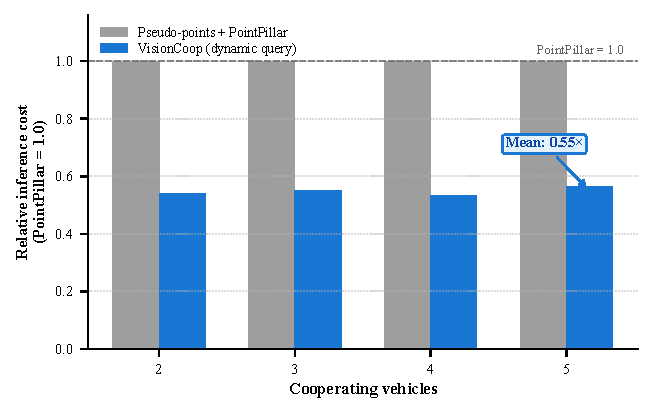
\includegraphics[width=\columnwidth]{figures/runtime_relative.pdf}
\caption{Relative average inference cost on the OPV2V test-set inference benchmark. PointPillar is normalized to 1.0 at each participant count; lower is better.}
\label{fig:runtime}
\end{figure}

\begin{table}[t]
\centering\small
\caption{Test image-compression results for \method{}. Payload is per vehicle at 10 Hz; AP evaluates end-to-end predicted-pose cooperative detection.}
\label{tab:compression}
\begin{tabular}{lrr}\toprule
Images & Mbps & AP$_{.5}$ (\%)\\\midrule
Original lossless & 99.59 & 44.52\\
JPEG Q95 & 22.80 & 40.23\\
JPEG Q80 & 10.81 & 38.49\\
JPEG Q60 & 7.09 & 37.16\\
JPEG Q40 & 5.41 & 36.41\\
Front/rear Q80, sides Q40 & 8.12 & 37.47\\\bottomrule
\end{tabular}
\end{table}

\textbf{Computation and inference comparison.} To avoid hardware-dependent timings, we report normalized average inference cost on OPV2V, with PointPillar normalized to 1.0 at each participant count. As shown in Fig.~\ref{fig:runtime}, \method{} uses 0.53--0.56$\times$ of the PointPillar cost (mean 0.55$\times$, 45.2\% lower). Bypassing pseudo-point conversion and pillar discretization achieves lower normalized cost; the figure represents relative efficiency rather than absolute latency.

\textbf{Image payload and compression.} Transmitting raw streams requires bandwidth management. Table~\ref{tab:compression} evaluates JPEG compression under 10\,Hz transmission. Uniform JPEG Q80 lowers per-vehicle payload from 99.59 to 10.81\,Mbps (>90\% reduction) while retaining 38.49\% AP$_{.5}$ (>84\% retention). Asymmetric compression (Q80 front/rear, Q40 sides) reaches 8.12\,Mbps with 37.47\% AP$_{.5}$, confirming viability over commercial V2X links.
